\makeatletter
\let\savedchap\@makechapterhead
\def\@makechapterhead{\vspace*{-3.5cm}\savedchap}

\setstretch{1.3}

\chapter{Multiplexer}
\section{Multiplexer 16:1}
\paragraph{Traccia}
Progettare, implementare in VHDL e testare mediante simulazione un multiplexer indirizzabile 16:1, utilizzando un approccio di progettazione per composizione a partire da multiplexer 4:1. 

\subsection{Architettura}
La soluzione prevede la connessione di 5 \textit{multiplexer} 4:1 secondo lo schema in Figura \ref{fig:mux_16_1}, in cui sono presenti due stadi:

\begin{itemize}
    \item al primo stadio si trovano quattro multiplexer a cui sono stati assegnati i bit più significativi del segnale di controllo;
    \item al secondo stadio è presente un solo multiplexer che raccoglie le uscite dello stadio precedente ed è controllato dai bit meno significativi del segnale di controllo;
\end{itemize}

\begin{figure}[H]
    \centering
    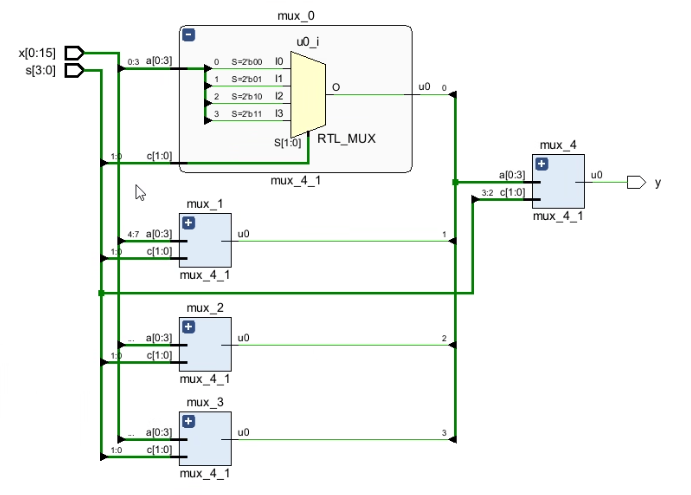
\includegraphics[width=16cm]{immagini/esercizio1/schema_1.1.png}
    \caption{Schema Multiplexer 16:1}
    \label{fig:mux_16_1}
\end{figure}

Il componente fondamentale dell'architettura è il \textit{multiplexer} 4:1 ed è stato realizzato con un approccio comportamentale come descritto nel listato in \ref{mux_4_1} con il costrutto \textit{case-when} inserito in un \textit{process} la cui lista di sensitività contiene sia la selezione che il dato.

\begin{lstlisting}[language=VHDL, label=mux_4_1, caption=Multiplexer 4:1]
library IEEE;
use IEEE.STD_LOGIC_1164.ALL;

entity mux_4_1 is
    Port ( 
        a: in STD_LOGIC_VECTOR (0 to 3);
        c: in STD_LOGIC_VECTOR (1 downto 0);
        u0: out STD_LOGIC
    );
end mux_4_1;

architecture behavioral of mux_4_1 is
begin
    process (a,c)
        begin  
        case c is 
            when "00" => u0 <= a(0);
            when "01" => u0 <= a(1);
            when "10" => u0 <= a(2);
            when "11" => u0 <= a(3);
            when others => u0 <= '-';
        end case;
    end process;
         
end behavioral;
\end{lstlisting}

L'architettura mostrata in Figura \ref{fig:mux_16_1} è stata realizzando componendo i singoli multiplexer, come illustrato nel listato \ref{mux_16_1}. In particolare, gli ingressi sono stati memorizzati in un vettore di $16 bit$ e le selezioni in uno da $4$, mentre l'uscita è rappresentata da un singolo segnale. Ai multiplexer elementari sono assegnati opportunamente i segnali di ingresso, ad esempio: al \textit{mux\_0}, sono stati assegnati i primi $4$ bit; al \textit{mux\_1} i successivi $4$ e così via. 

\begin{lstlisting}[language=VHDL, label=mux_16_1 caption=Multiplexer 16:1]
library IEEE;
use IEEE.STD_LOGIC_1164.ALL;

entity mux_16_1 is
  Port ( 
      x: in STD_LOGIC_VECTOR (0 to 15);
      s: in STD_LOGIC_VECTOR (3 downto 0); 
      y: out STD_LOGIC
  );
end mux_16_1;

architecture structural of mux_16_1 is
   component mux_4_1 is
     Port ( 
        a: in STD_LOGIC_VECTOR (0 to 3);
        c: in STD_LOGIC_VECTOR (1 downto 0);
        u0: out STD_LOGIC
     );
   end component;
signal k : STD_LOGIC_VECTOR (0 to 3);
signal inputs: STD_LOGIC_VECTOR(0 to 15);
signal selections: STD_LOGIC_VECTOR(3 downto 0);
signal output: STD_LOGIC;

begin
 mux_0: mux_4_1 
  Port map(
    a(0 to 3) => x(0 to 3),
    c(1 downto 0) => s(1 downto 0),
    u0=>k(0)  
  );
  
 mux_1: mux_4_1 
  Port map(
    a(0 to 3) => x(4 to 7),
    c(1 downto 0) => s(1 downto 0),
    u0=>k(1)  
  );

 mux_2: mux_4_1 
  Port map(
    a(0 to 3) => x(8 to 11),
    c(1 downto 0) => s(1 downto 0),
    u0=>k(2)  
  );
  
 mux_3: mux_4_1 
  Port map(
    a(0 to 3) => x(12 to 15),
    c(1 downto 0) => s(1 downto 0),
    u0=>k(3)  
  );

  mux_4: mux_4_1
  Port map (
    a(0 to 3) => k(0 to 3),
    c(1 downto 0) => s(3 downto 2),
    u0 => y
  );
   
end structural;
\end{lstlisting}


\subsection{Testing}
Sono stati esaminati due casi di test, in cui con uno stesso segnale di ingresso sono stati fatti variare i bit di controllo. Per ogni test sono stati verificati gli output attesi.
L'input mette a $1$ le linee di ingresso $6,7,8,9$.\\
Per il primo caso di test la selezione è "0110" per cui ci si aspetta correttamente l'output in $1$.\\
Per il secondo caso di test la selezione è "0001" per cui ci si aspetta correttamente l'output pari $0$.

Nel listato \ref{mux_16_1}, è riportato il \textit{testbench} utilizzato per testare il componente realizzato.

\begin{lstlisting}[language=VHDL, label=mux_16_1, caption=Testbench mux 16:4]
library IEEE;
use IEEE.STD_LOGIC_1164.ALL;

entity mux_16_1_TB is
end mux_16_1_TB;

architecture Behavioral of mux_16_1_TB is

  component mux_16_1 is
    Port ( 
      x: in std_logic_vector(0 to 15);
      s: in std_logic_vector(3 downto 0); 
      y: out std_logic
    );
  end component;

signal inputs: std_logic_vector(0 to 15);
signal selections: std_logic_vector(3 downto 0);
signal output: std_logic;

begin
  --Unit Under Test
  uut: mux_16_1
    Port map ( 
      x => inputs,
      s => selections,
      y => output
    );
  test_bench: process
  begin
    -- Caso test 1
    wait for 10 ns;
    inputs <= "0000001111000000";
    selections <= "0110";
    wait for 10 ns;
    assert output <= '1';
    report "errore_1" severity failure;

    -- Caso test 2
    wait for 20 ns;
    inputs <= "0000001111000000";
    selections <= "0001";
    wait for 10 ns;
    assert output <= '0';
    report "errore_2" severity failure;
  wait;
  end process;
end Behavioral;
\end{lstlisting}

\begin{figure}[H]
    \centering
    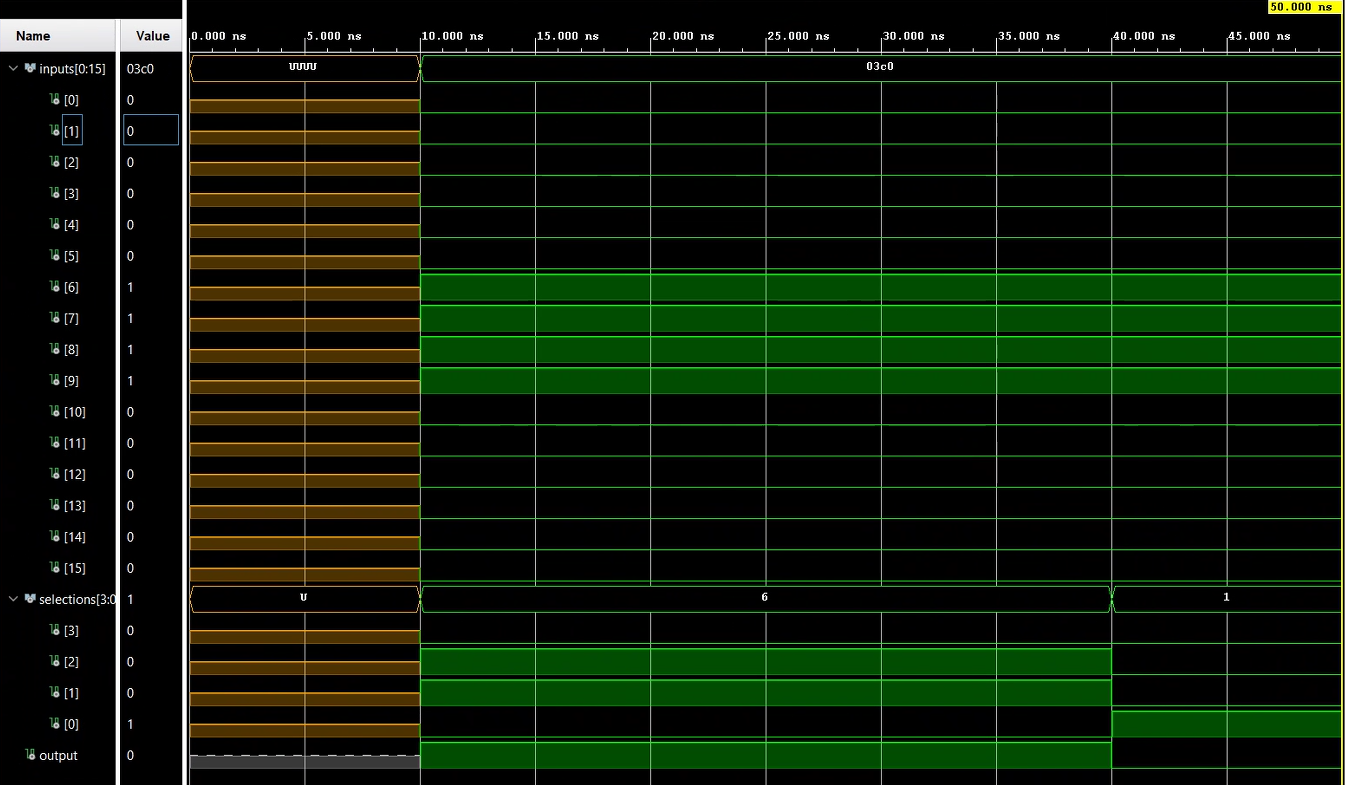
\includegraphics[width=16cm]{immagini/esercizio1/output_simulazione_1.1.png}
    \caption{Simulazione}
    \label{fig:notebook}
\end{figure}

\section{Rete 16:4}
\paragraph{Traccia}
Utilizzando il componente sviluppato al punto precedente, progettare, implementare in VHDL e testare mediante simulazione una rete di interconnessione a 16 sorgenti e 4 destinazioni.

\subsection{Architettura}

Come descritto nello schema in Figura \ref{fig:16_4}, per costruire una rete 16:4 è necessario collegare in cascata un \textit{multiplexer 16:1} e un \textit{de-multiplexer 1:4}  ai quali bisogna assegnare, in maniera opportuna, gli ingressi di selezione. Infatti, al \textit{multiplexer} sono stati assegnati i $4$ bit più significativi del vettore della selezione, mentre al \textit{de-multiplexer} corrispondono i $2$ bit meno significativi. 

L'architettura si presenta come segue:
\begin{figure}[H]
    \centering
    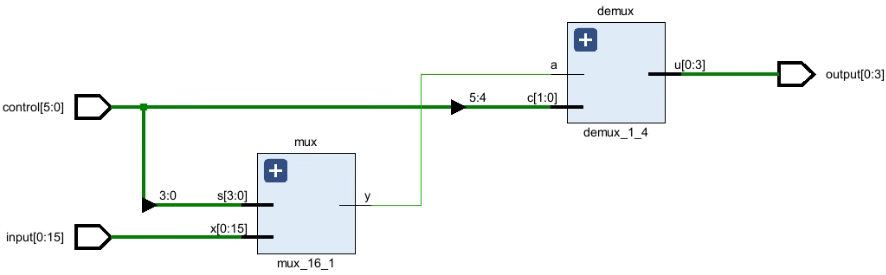
\includegraphics[width=16cm]{immagini/esercizio1/schema_1.2.png}
    \caption{Schema architettura}
    \label{fig:16_4}
\end{figure}

Analogamente al \textit{multiplexer} nel paragrafo precedente, il \textit{de-multiplexer} è implementato in un \textit{process} con il costrutto \textit{case-when}, come illustrato nel listato \ref{demux_1_4}.

\begin{lstlisting}[language=VHDL, label=demux_1_4, caption=Demultiplexer 1:4]
library IEEE;
use IEEE.STD_LOGIC_1164.ALL;

entity demux_1_4 is
    Port (
        a: in STD_LOGIC;
        c: in STD_LOGIC_VECTOR (1 downto 0);
        u: out STD_LOGIC_VECTOR(0 to 3)
    );
end demux_1_4;

architecture Behavioral of demux_1_4 is

begin
    process(a,c)
        begin
        case c is 

        when "00" => 
            u(0) <= a;
            u(1) <= '0';
            u(2) <= '0';
            u(3) <= '0';
        
        when "01" => 
            u(0) <= '0';
            u(1) <= a;
            u(2) <= '0';
            u(3) <= '0';
            
        when "10" => 
            u(0) <= '0';
            u(1) <= '0';
            u(2) <= a;
            u(3) <= '0';
            
        when "11" => 
            u(0) <= '0';
            u(1) <= '0';
            u(2) <= '0';
            u(3) <= a;

        when others => 
            u(0)<= '-';
            u(1)<= '-';
            u(2)<= '-';
            u(3)<= '-';
        end case;
    end process;
end Behavioral;
\end{lstlisting}

Nel listato \ref{rete_16_4} è mostrata l'implementazione della soluzione. In particolare, i due componenti dell'architettura sono collegati mediante il segnale \textit{k}. 

\begin{lstlisting} [language=VHDL, label=rete_16_4, caption=Rete 16:4]
library IEEE;
use IEEE.std_logic_1164.ALL;

entity Rete_16_4 is 
  Port (  
    input: in std_logic_vector(0 to 15);
    control: in std_logic_vector(5 downto 0); 
    output: out std_logic_vector(0 to 3)
  );
end Rete_16_4;

architecture Structural of Rete_16_4 is

  component mux_16_1 is
    Port ( 
      x: in std_logic_vector(0 to 15);
      s: in std_logic_vector(3 downto 0); 
      y: out std_logic
    );
  end component;

  component demux_1_4 is
    Port (
      a: in std_logic;
      c: in std_logic_vector (1 downto 0);
      u: out std_logic_vector(0 to 3)
     );
  end component;

 signal k : std_logic;
 begin
   mux: mux_16_1 port map(
       x(0 to 15) => input(0 to 15),
       s(3 downto 0) => control(3 downto 0),
       y=>k
     );
    
   demux: demux_1_4 port map(
       a => k,
       c(1 downto 0) => control(5 downto 4),
       u(0 to 3)=>output(0 to 3)
     );

 end Structural;
\end{lstlisting}


\subsection{Testing}
Per dimostrare il corretto funzionamento del componente è stato progettato un \textit{testbench} (riportato per intero nel listato \ref{tb_16_4}) con 3 casi di test in cui sono assegnati degli \textit{input} e viene verificato un \textit{assert} con l'\textit{output} atteso. Infine, in Figura \ref{fig:sim_1_2} è mostrata l'esecuzione della testbench mediante una simulazione.

\begin{lstlisting}[language=VHDL, label=tb_16_4, caption=Testbench Rete 16:4]
library IEEE;
use IEEE.STD_LOGIC_1164.ALL;

entity Rete_16_4_TB is
end Rete_16_4_TB;

architecture Behavioral of Rete_16_4_TB is

component Rete_16_4 is
  Port (  
    input: in std_logic_vector(0 to 15);
    control: in std_logic_vector(5 downto 0); 
    output: out std_logic_vector(0 to 3)
  );
end component;

signal inputs_16_4: std_logic_vector(0 to 15);
signal selections_16_4: std_logic_vector(5 downto 0);
signal output_16_4: std_logic_vector(0 to 3);
begin

--Unit Under Test
  uut: Rete_16_4
    Port map ( 
      input=> inputs_16_4,
      control => selections_16_4,
      output => output_16_4
    );

test_bench: process
begin

  wait for 100 ns;

  -- Caso di test 1
  inputs_16_4 <= "0000001111000000";
  selections_16_4 <= "011001";
  wait for 10 ns;
  assert output_16_4(1) = '1' report "errore0" severity failure;

  -- Caso di test 2
  wait for 10 ns;
  inputs_16_4 <= "1111111111111111";
  selections_16_4 <= "111110";
  wait for 10 ns;
  assert output_16_4(3) = '1' report "errore1" severity failure;

  -- Caso di test 3
  wait for 10 ns;
  inputs_16_4 <= "0000001111000000";
  selections_16_4 <= "011001";
  wait for 10 ns;
  assert output_16_4(1) = '0' report "errore2" severity failure;

  wait;

end process;
end Behavioral;
\end{lstlisting}


\begin{figure}[H]
    \centering
    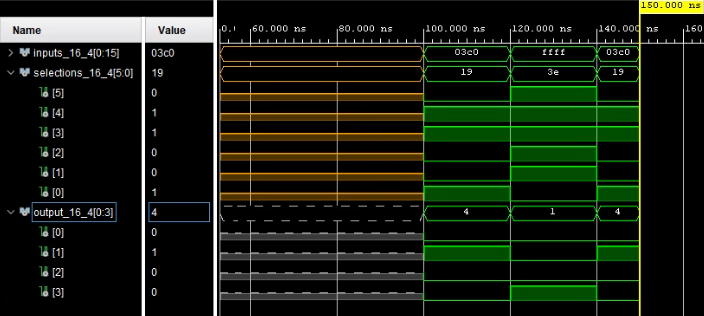
\includegraphics[width=16cm]{immagini/esercizio1/output_simulazione_1_2.png}
    \caption{Simulazione}
    \label{fig:sim_1_2}
\end{figure}



\section{Sintesi su scheda}
\paragraph{Traccia}
Sintetizzare ed implementare su board il progetto della rete di interconnessione sviluppato al punto 1.2, utilizzando gli switch per fornire gli input di selezione e i led per visualizzare i 4 bit di uscita. Per quanto riguarda i 16 bit dato in input, essi possono essere precaricati nel sistema oppure immessi anch’essi mediante switch, sviluppando in questo secondo caso un’apposita rete di controllo per l’acquisizione.

\subsection{Implementazione}
Per la risoluzione dell'esercizio si è deciso di integrare la soluzione precedente. In particolare è stata implementata una rete di controllo, che serve ad effettuare l'acquisizione del dato in ingresso dagli \textit{switch} della scheda e ad avviare la trasmissione con un pulsante.

\subsubsection{Acquisizione dati}
Per acquisire i dati dalla \textit{board} è stata effettuata la mappatura degli \textit{switch} con il vettore dei segnali di ingresso ed è stato integrato l'esercizio 1.2 con una rete di controllo implementata con un FSM (illustrata in Figura \ref{fig:cu_1_3}). Questa introduzione trasforma la macchina da puramente combinatoria a sequenziale, con la necessità di introdurre il \textit{clock}. Inoltre, l'impulso del pulsante fisico deve essere ripulito da un \textit{debouncer} per evitare che duri più di un colpo di \textit{clock}.


\begin{figure}[H]
    \centering
    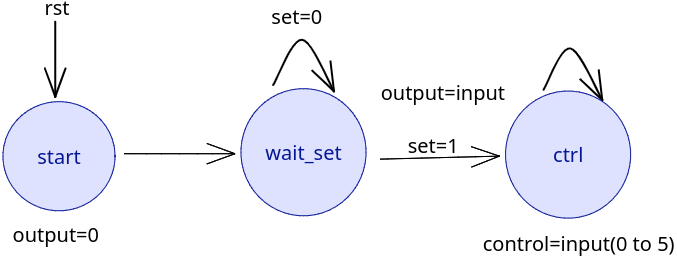
\includegraphics[width=14cm]{immagini/esercizio1/automa_1.3.png}
    \caption{Rete di controllo}
    \label{fig:cu_1_3}
\end{figure}

Nel listato \ref{dbncr} è stata riportata per semplicità solo l'interfaccia utilizzata del componente \textit{ButtonDebouncer}. In particolare, attraverso i parametri di \textit{clock} e tempo di rimbalzo crea un contatore che controlla che la pressione del pulsante sia costante in modo tale da eliminare leggere perturbazioni che potrebbero portare ad avere comportamenti errati.

\begin{lstlisting}[language=VHDL, label=dbncr, caption=Interfaccia ButtonDebouncer]
entity ButtonDebouncer is
   generic(  CLK_period: integer := 10; -- periodo del clock in nanosec
             btn_noise_time: integer := 10000000 --durata dell'oscillazione in nanosec  );
    Port ( RST : in STD_LOGIC;
           CLK : in STD_LOGIC;
           BTN : in STD_LOGIC; 
           CLEARED_BTN : out STD_LOGIC);
end ButtonDebouncer;
\end{lstlisting}